\chapter{Background}
\label{background}

This chapter provides background information by contributing to a basic
understanding of the field of software evolution, the assessment of
survivability and success of OSS projects, and wavelet analysis.

\section{Software evolution}
The analogy of the term \emph{evolution }\rm in the field of software
engineering was first used by \citet{lehman} in his laws of software evolution.
Software does not evolve by intrinsic feedback loops like evolution in plants
and animals, but by extrinsic feedback that comes from the operational domain.

\paragraph{}
\citeauthor{lehman} identified eight laws that are the driving factors of
changes in software systems. These laws can be roughly categorised into two
categories: laws related to the product (e.g., source code, and internal
quality), and laws related to the process (e.g., organisation, development
process, business requirements and user satisfaction).

\paragraph{}
The laws related to the software process tell us that in order for a software
system to stay useful and satisfactory, it needs to keep changing according to
users' needs. What needs to change is fed through the feedback system.

On average and in terms of activity, the organisation of a software development
process does not change much during a product's life time; \citeauthor{lehman}'s
fourth law: Conservation of Organisational Stability.

\paragraph{}
The laws related to the software product tell us that as the source code of the
software system changes, its complexity will increase and its quality will
decline unless proper actions are taken to maintain it or reduce the complexity
and improve its quality. However, the contents of the product will be
statistically invariant during the active life time of a product.

\paragraph{}
\citeauthor{lehman}'s laws of software evolution are valid for both closed
source software and open-source software. These laws form the foundation of
what we understand as software evolution.

\paragraph{}
The evolution of a software system comprises various measures on different
moments in time. For instance, the lines of code metric over a project's life
time is a way to measure the evolution of lines of code in a software project.



\section{Project survivability}
%% perhaps restructure in Project success, and Project survivability %%
In a study by \citet{samoladas2010} a method for survival analysis on OSS
projects was proposed. The authors used duration data regarding Free/Libre
Open-Source Software (FLOSS) projects to predict the survivability of the
projects by examining their duration, combined with other characterstics such
as application domain and number of committers. These metrics give insight in
the survivability chances of a project. It was also found that adding a
developer to the team of contributors increased the survivability of the
project substantially.

The authors proposed two main research issues to be addressed in the future.
The first one is to add more projects to the study with possibly a different
categorisation. And second, the effects of more project parameters, such as
programming language should be examined. This is not trivial since typically
more than one language is used in each project.

\paragraph{}
A study by \citet{raja2012} on defining a measure of OSS project survivability.
They have been looking for vitality of OSS projects: the ability of a project
to grow and maintain its structure in the presence of perturbations. They
identified three dimensions of project viability: vigor -- the ability of a
project to grow --, resilience -- the ability of a project to recover from
disturbances --, and organisation -- the structure exhibited in the project.
These dimensions represent three distinct characteristics of project viability.

This measure is of use to determine survivability of a project, however, it is
a snapshot of a single point in time. It does not take into account the events
prior to this point in time, nor does it enable prediction of survivability in
the near future. Therefore, it can be challenging to get an objective view on a
project's survivability as a representative point in time has to be selected.

\paragraph{}
\citet{crowston2003} identified measures that can be applied to assess the
success of OSS projects. The authors used the ``Model of Information Systems
Success'' by \citet{delone1992} to evaluate OSS project success. The aspects
identified by \citeauthor{delone1992} are elaborated; output of systems
development -- it is believed that a project that has a high frequency of
releases is healthy --, process of systems development -- the number of
developers, the individual level of activity, and cycle time (time between
releases) --, and project effects -- employment opportunities of the
contributors, individual reputation, and knowledge creation. In this study it
was found that many of these aspects are indicators of OSS project success.

Although the cycle time is an aspect that could be measured automatically, the
other aspects such as employment opportunities, reputation, and knowledge
creation are very hard to get into numbers and therefore hard to automate.

\paragraph{}
Another study conducted by \citet{crowston2006} extends the previous study by
using Free/Libre Open-Source Software (FLOSS) projects. In addition to what was
found in the previous study, they had found that the number of developers as a
simple count of developers is a flawed number as it aggregates the number of
developers leaving and the number of developers joining a project. A 'churn' of
the developers or a 'tenure' of individuals would be more appropriate.

\paragraph{}
A study conducted by \citet{wang2012} has shown that warning signs can be found
in six crucial factors of OSS projects success: developer participation effort,
developer service quality, software license restrictiveness, targeted users,
community social network ties, and community quality of social ties.

\paragraph{}
\citet{karus2013} explored a method known as \emph{wavelet analysis }\rm to
analyse software evolution data. The wavelet analysis interprets evolution data
as a series of signals and is able to find sequences in this signal. The
sequences of multiple projects can be compared in order to find recurring
patterns. Karus was able to detect 998 similar patterns across 27 OSS projects.
He concluded that wavelet analysis can be a powerful tool for identifying
evolutionary events.





\section{Wavelet analysis}
\label{wavelet_analysis}
A wavelet is a portion of a continuous-time signal (also known as waveform).
Opposed to the continuous wave which has infinite duration, the wavelet has a
finite duration.

The analysis of waves is being used in many fields, such as, economics,
seismology, (astro-)physics, and computer science.

\subsection{Waveforms}
A waveform, or wave, is a signal (time-series) in a two-dimensional space.
Waveforms are used to model many types of signals, such as audio,
electromagnetic (light), gravitational, and quantum mechanical waves.

\paragraph{}
In many models of waveforms the two dimensions typically represent the time and
frequency domains. An audio signal is an example of a waveform modeled that way.

In visualisations of waveforms, the time domain is often plotted on the
horizontal axis, and the frequency domain on the vertical axis. In the example
of an audio wave (see Figure \ref{figure:wave}), the frequency domain may
represent the amplitude, or the frequency, and the time the duration of the
amplitude or frequency value.

\begin{figure}[h]
\caption{Example of an audio wave}\label{figure:wave}
\centering
	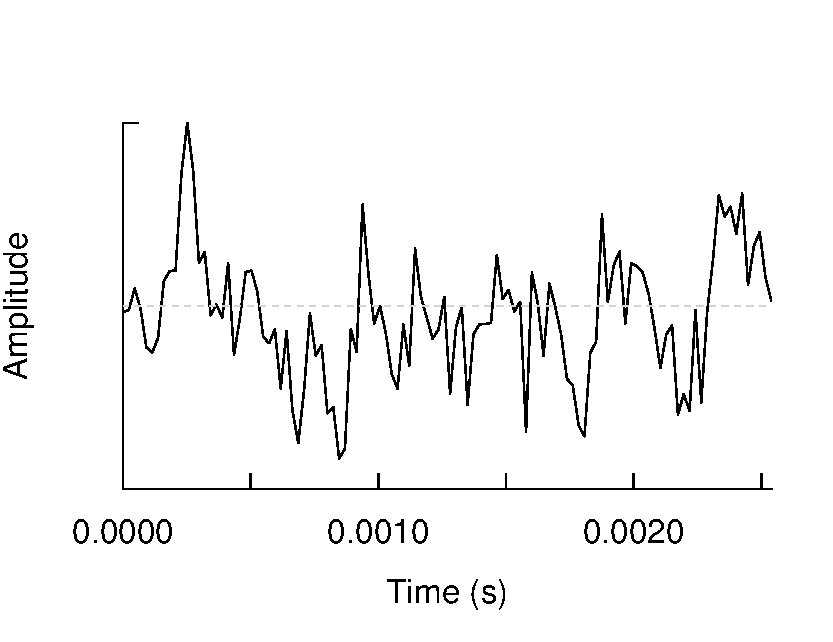
\includegraphics[height=192pt]{images/pink_audio.pdf}
\end{figure}

However, the time domain is not specifically bound to time intervals only. A
less intuitive, but realistic approach would be to model amplitude in the time
domain. That way the frequency relation to amplitude of a signal can be
analysed, but the time information is lost.

\subsection{Discrete wavelet transformation}
To be able to analyse and compare different wavelets, we need a way to scale
the signal. Discrete wavelet transformation is the operation of applying a
filter function (also known as 'filter'), or set of filter functions (also known
as 'filter bank') to the wavelet. This is a way of sampling the signal at
different intervals giving a natural means of scaling the signal
\cite{karus2013}.

\paragraph{}
Wavelet analysis is similar to Fourier analysis with the difference that
wavelet transform deals with time and frequency information, and Fourier
transform deals with frequency information only. Wavelet analysis is the
transformation of signals (time-series) by decomposing the signal into
wavelet/shift coefficients, and scaling/filter coefficients based on wavelet
functions (filters) \cite{karus2013}.

Shifting/translating is the operation of moving the wavelet in the time
domain producing scale/filter coefficients, and requires frequency resolution.
Filtering/dilating is the operation of scaling the the wavelet in the frequency
domain producing wavelet/shift coefficients, and requires time resolution.
These operations are illustrated in Figure \ref{figure:shifting} and Figure
\ref{figure:filtering} respectively.

The decomposition can be repeated on the scale/filter coefficients until the
number of resulting wavelet/shift coefficients is smaller than the filter
length \cite{graps}. The filter length is a property of the filter function
being used.

\begin{figure}[h]
\caption{Shifting/translating a wavelet}\label{figure:shifting}
\caption*{\\[1em]\emph{Left: the input signal 1 second sine wave\\ Right: the
signal shifted 1 second to the right}\rm}
\centering
	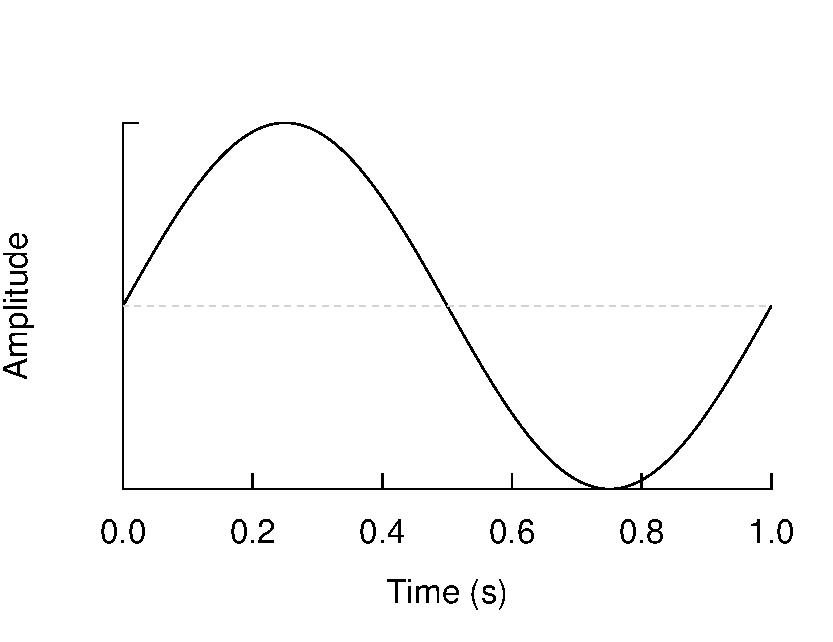
\includegraphics[width=196pt]{images/sine_full.pdf}
	\hspace{1em}
	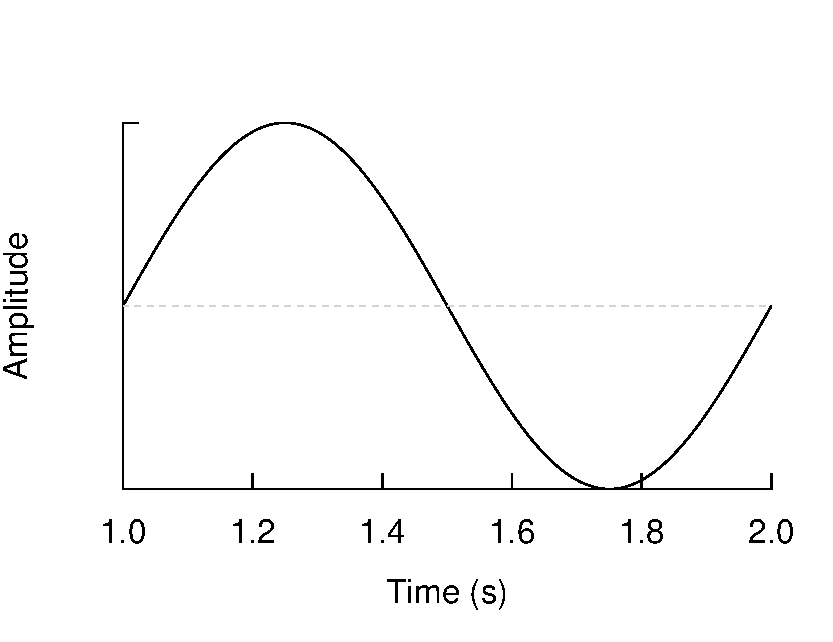
\includegraphics[width=196pt]{images/sine_shifted.pdf}
\end{figure}
\vspace{1em}
\begin{figure}[h]
\caption{Filtering/dilating a wavelet}\label{figure:filtering}
\caption*{\\[1em]\footnotesize\emph{Left: the input signal 1 second sine wave\\
Right:
the signal scaled to a 2 second sine wave}\rm}
\centering
	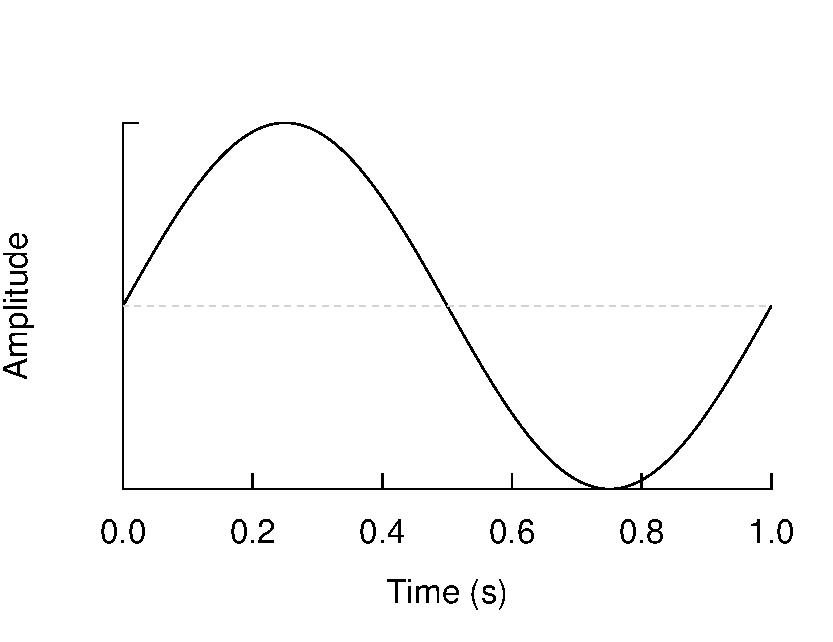
\includegraphics[width=196pt]{images/sine_full.pdf}
	\hspace{1em}
	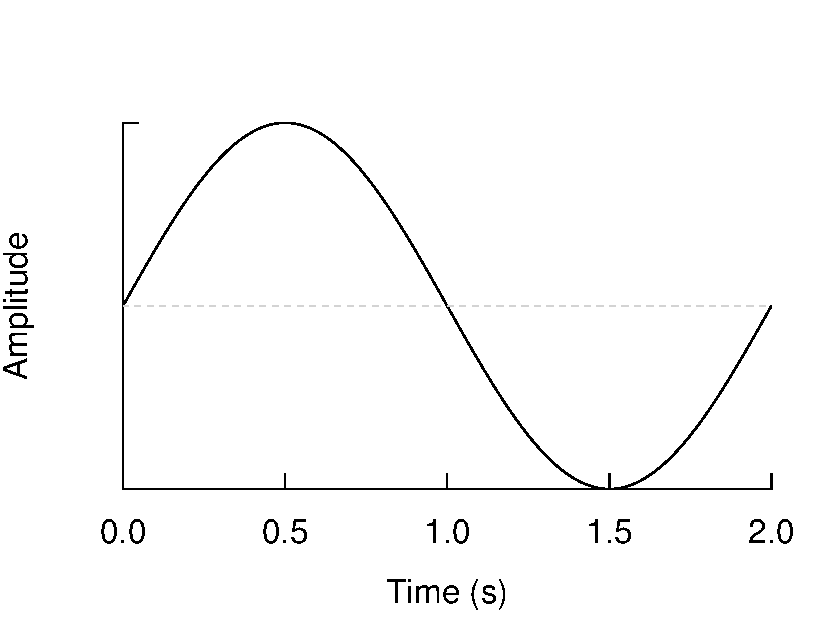
\includegraphics[width=196pt]{images/sine_scaled.pdf}
\end{figure}

\paragraph{}
Wavelet transform has proven important in signal processing thanks to its
inherent properties which allow comparisons at different scales and shifts.
Compared to other time series analysis techniques, the main advantages of
wavelet transformations in the analysis of signals are \cite{karus2013}:
\begin{itemize}
	\item Wavelet/shift coefficients allow fuzzy matching as differences in details
	are 'smoothed out'.
	\item Filter/scale coefficients allow detection of small anomalies in series.
	\item Transform levels make series of different lengths or scale comparable.
\end{itemize}

\subsection{Wavelet functions}
A wavelet function is a function that defines a wavelet. In general, a wavelet
function is any operation on an existing wavelet \cite{wadkar}. Many wavelet
functions exist and differ largely in complexity and applicability depending on
the signal of interest.

A wavelet can be defined in the following ways, given that $T$ is the set of
time values of the signal, and $F$ the set of frequency values of the signal.
\begin{description}
	\item[Wavelet function (mother wavelet)] \hfill \\ $\Psi: T \rightarrow
	F$\\ $\Psi(t) = f$, such that $t \in T$ and $f \in F$.\\
	This function maps $T$ onto $F$ and thus produces the shape of the wavelet.

	\item[Scaling function (father wavelet)] \hfill \\ $\Phi: F \rightarrow
	T$\\ $\Phi(f) = t$, such that $t \in T$ and $f \in F$.\\
	This function maps $F$ onto $T$ and thus produces the scale of the wavelet.

	\item[Scaling filter] \hfill \\ A low-pass filter of length $2N$ and sum $1$.
	A high-pass filter can be calculated as the quadrature mirror filter of the
	low-pass filter. All Daubechies wavelets can be defined by the scaling filter.
\end{description}

\subsection{Haar wavelet}
The Haar wavelet is a member of the Daubechies family of wavelets, based on the
work of the Belgian mathematician Ingrid Daubechies. The Daubechies wavelets is
a family of orthogonal wavelets defining a discrete wavelet transform. All
wavelets of the Daubechies family can be entirely defined by their scaling
filter. The Haar wavelet has a filter of length 2 and is therefore also
referenced to as the Daubechies-2 (D2) filter. It is the simplest wavelet of
the Daubechies family.

\begin{figure}[H]
\caption{The Haar functions}\label{figure:haar}
\centering
\caption*{\\[1em]\footnotesize\textit{(a) The Haar wavelet function (mother
wavelet)}}
\[
\begin{aligned}
\Psi(t) = \left\{
	\begin{array}{r r}
		1  & \quad   0 \leq t < 1/2, \\
		-1 & \quad 1/2 \leq t < 1, \\
		0  & \quad \text{otherwise.}
	\end{array}
\right.
\end{aligned}
\qquad
\raisebox{-15mm}{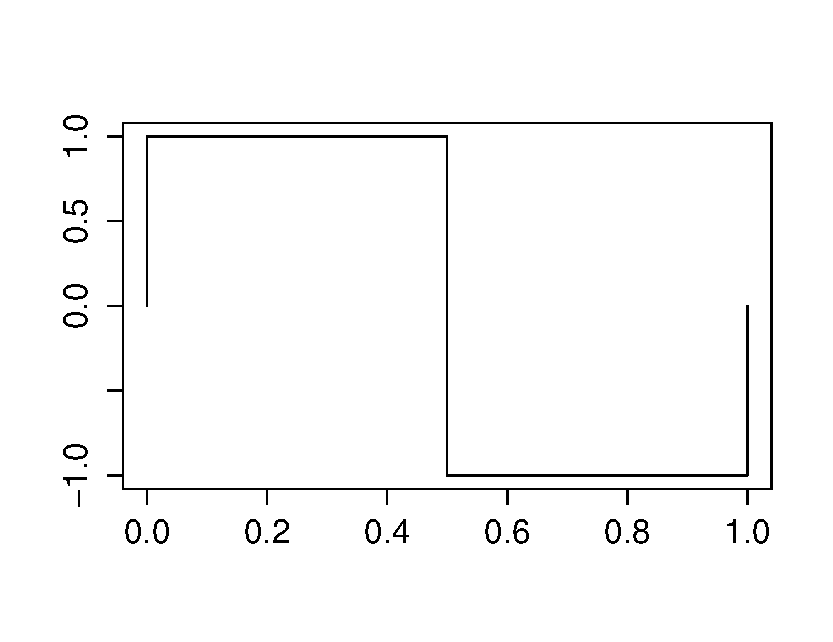
\includegraphics[height=128pt]{images/haar.pdf}}
\]
\caption*{\footnotesize\textit{(b) The Haar scaling function (father wavelet)}}
\[
\Phi(t) = \left\{
	\begin{array}{r r}
		1 & \quad 0 \leq t < 1, \\
		0 & \quad \text{otherwise.}
	\end{array}
\right.
\]
\end{figure}


\paragraph{}
In 1910, the Hungarian mathematician Alfred Haar introduced Haar functions. The
Haar transform is one of the earliest examples of what is known now as a
compact, dyadic, orthonormal wavelet transform \cite{stankovic}. The Haar
function is the simplest and oldest orthonormal wavelet with compact support.

\subsection{Wavelet transformation using the Haar filter}
The Haar filter function varies in scale by splitting the input signal using
different scale sizes. If we have a signal over the domain from 0 to 1, we can
divide the signal into two wavelets that range from 0 to $1/2$ and from
$1/2$ to 1. Then we can divide the signal again giving four wavelets that range
from 0 to $1/4$, from $1/4$ to $2/4$, from $2/4$ to $3/4$, and from $3/4$ to 1
\cite{graps}. This decomposition can be repeated as long as the time resolution
of the original signal allows.

In each scaling or filtering step (i.e., decomposition) the Haar function adds
more detail to the wavelets in the current level. The Haar filter captures the
differences between scale levels. The resulting coefficients can be used to
compare signals regardless of scale and length \cite{graps}.

\paragraph{}
Wavelet transformation with the Haar filter is widely used. For example, as a
way of digitalising an analogue signal in A-D converters, pattern recognition,
face recognition, image processing, data coding, multiplexing, digital
filtering, digital speech processing, voice controlled computing devices,
robotics, compression mechanisms, and other kinds of digital signal processing.

\begin{comment}
- Literature study
- Software evolution
- Project success
- Project survivability

This chapter contains all the information needed to put the thesis into
context. It is common to use (a revised version) of your literature survey for
this purpose.
It is important to refer from your text to sources you have used, as listed in
your bibliography section (appendix). For example, “XP is a recent agile
development method [1]” is a common style of doing this, where the following
entry would be included in your bibliography:
[1] K. Beck, E. Gamma, Test infected: Programmers love writing tests, Java
Report 3 (7) (1998) 51–56.
If you want to refer to books you have read as part of the curriculum, you can
also do so in this way.
Have a look at Chapter 2 of this example thesis at Paul’s
homepage\footnote{http://homepages.cwi.nl/~paulk/thesesMasterSoftwareEngineering/2006/RichardKettelerij.pdf}.
\end{comment}